\section{Experimental Results}

\subsection*{Evaluation Metrics}
We use two metrics to measure model accuracy, using the cardiologist committee
annotations as the ground truth.

\textbf{Sequence Level Accuracy (F1):} We measure the average overlap between
the prediction and the ground truth sequence labels. For every record, a model
is required to make a prediction approximately once per second (every 256
samples). These predictions are compared against the ground truth annotation.

\textbf{Set Level Accuracy (F1):} Instead of treating the labels for a record
as a sequence, we consider the set of unique arrhythmias present in each 30
second record as the ground truth annotation. Set Level Accuracy, unlike
Sequence Level Accuracy, does not penalize for time-misalignment within a
record. We report the F1 score between the unique class labels from the ground
truth and those from the model prediction.

In both the Sequence and the Set case, we compute the metrics for each class
separately. We then compute aggregate results for AUC and F1 as the
class-frequency weighted mean.

\subsection*{Model and Cardiologist Performance}

We assess the cardiologist performance on the test set. Recall that each of the
records in the test set has a ground truth label from a committee of three
cardiologists as well as individual labels from a disjoint set of 6 other
cardiologists. To assess cardiologist performance for each class, we take the
average of all the individual cardiologist scores using the group label as the
ground truth annotation.

\begin{table}
\centering
\begin{small}
\begin{tabular}{r l l}
\toprule
                               & Sequence AUC & Set AUC \\
\midrule
Atrial Fibrillation \& Flutter & 0.975 & 0.959 \\
Atrio-ventricular Block        & 0.989 & 0.981 \\
Bigeminy                       & 0.998 & 0.997 \\
Ectopic Atrial Rhythm          & 0.908 & 0.935 \\
Idioventricular Rhythm         & 0.995 & 0.986 \\
Junctional Rhythm              & 0.985 & 0.980 \\
Noise                          & 0.985 & 0.958 \\
Sinus Rhythm                   & 0.976 & 0.981 \\
Supraventricular Tachycardia   & 0.972 & 0.940 \\
Trigeminy                      & 0.999 & 0.997 \\
Ventricular Tachycardia        & 0.995 & 0.981 \\
Wenckebach                     & 0.982 & 0.981 \\
\midrule
   Average                     & 0.979               & 0.974 \\
\bottomrule
\end{tabular}
\end{small}
\caption{The model AUC scores for each rhythm class and in aggregate.}
\label{tab:arrhythmias:model_auc}
\end{table}

Table~\ref{tab:arrhythmias:model_auc} gives the per class and aggregate AUC
scores. Our model achieves an AUC of greater than 0.90 for each of the 12
rhythm diagnoses, with an average AUC of 0.97. We also compute the sensitivity
at a specifity of 0.9 and vice versa in~\ref{tab:arrhythmias:sens_spec}.

\begin{table}
\centering
\begin{small}
\begin{tabular}{r l l}
\toprule
             & Sensitivity       & Specificity  \\
\midrule
Atrial Fibrillation \& Flutter & 0.923 & 0.914 \\
Atrio-ventricular Block        & 0.991 & 0.964 \\
Bigeminy                       & 1.000 & 0.997 \\
Ectopic Atrial Rhythm          & 0.754 & 0.665 \\
Idioventricular Rhythm         & 0.990 & 0.990 \\
Junctional Rhythm              & 0.982 & 0.959 \\
Noise                          & 0.965 & 0.968 \\
Sinus Rhythm                   & 0.934 & 0.946 \\
Supraventricular Tachycardia   & 0.958 & 0.925 \\
Trigeminy                      & 1.000 & 0.999 \\
Ventricular Tachycardia        & 1.000 & 0.981 \\
Wenckebach                     & 0.977 & 0.956 \\
\bottomrule
\end{tabular}
\end{small}
\caption{The maximum model sensitivity with specificity greater than 0.9 and
         vice versa.}
\label{tab:arrhythmias:sens_spec}
\end{table}

\begin{table}
\centering
\begin{small}
\begin{tabular}{r c c c c}
\toprule
    & \multicolumn{2}{c}{Sequence F1} & \multicolumn{2}{c}{Set F1} \\
\cmidrule{2-5}
 & Model & Cardiol. & Model & Cardiol. \\
\midrule
Atrial Fibrillation \& Flutter & 0.802 & 0.679 & 0.817 & 0.687 \\
Atrio-ventricular Block        & 0.850 & 0.769 & 0.830 & 0.756 \\
Bigeminy                       & 0.896 & 0.837 & 0.870 & 0.849 \\
Ectopic Atrial Rhythm          & 0.537 & 0.476 & 0.545 & 0.529 \\
Idioventricular Rhythm         & 0.751 & 0.632 & 0.818 & 0.720 \\
Junctional Rhythm              & 0.640 & 0.684 & 0.778 & 0.674 \\
Noise                          & 0.852 & 0.768 & 0.704 & 0.689 \\
Sinus Rhythm                   & 0.886 & 0.847 & 0.934 & 0.907 \\
Supraventricular Tachycardia   & 0.458 & 0.449 & 0.630 & 0.556 \\
Trigeminy                      & 0.909 & 0.843 & 0.870 & 0.816 \\
Ventricular Tachycardia        & 0.520 & 0.566 & 0.653 & 0.769 \\
Wenckebach                     & 0.714 & 0.593 & 0.806 & 0.736 \\
\midrule
Average	                       & 0.808 & 0.750 & 0.809 & 0.778 \\
\bottomrule
\end{tabular}
\end{small}
\caption{The F1 score for the sequence and set-level metrics comparing the
         model and the average of six individual cardiologist to the committee
         consensus ground truth.}
\label{tab:arrhythmias:model_cardiologist_f1}
\end{table}

Table~\ref{tab:arrhythmias:model_cardiologist_f1} shows the breakdown of both
cardiologist and model sequence and set F1 across the different rhythm classes.
The model outperforms the average cardiologist performance on most rhythms,
noticeably outperforming the cardiologists in the AV Block set of arrhythmias
which includes Mobitz I (Wenckebach), Mobitz II and complete heart block (both
categorized as Atrio-ventricular Block). This is especially useful given the
severity of second and third degree heart block and the importance of
distinguishing these two from Wenckebach which is usually considered benign.
The model also outperforms the cardiologist average accross all rhythm classes
for both the sequence and set F1 score.

\begin{figure}
\centering
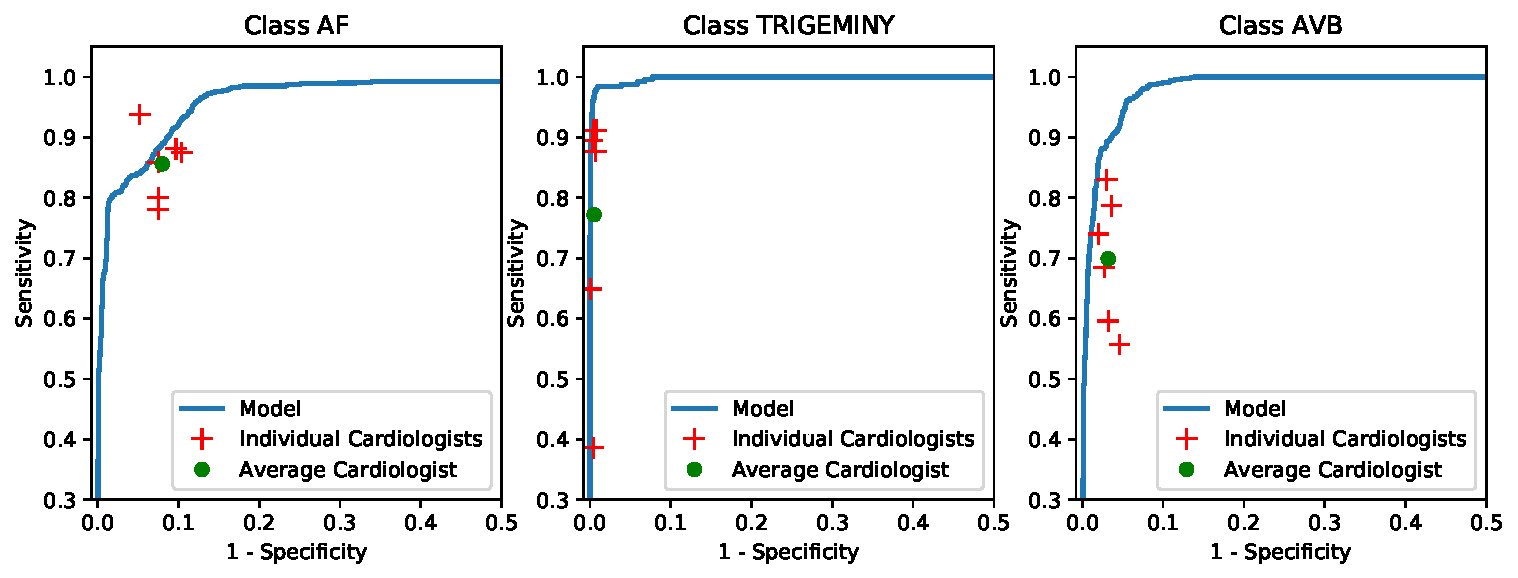
\includegraphics[width=1.0\textwidth]{arrhythmias/figures/roc_curve.pdf}
\caption{Receiver operating characteristic curves at the sequence level for
    atrial fibrillation and flutter (AF), trigeminy and atrioventricular block
    (AVB).}
\label{fig:arrhythmias:roc_curve}
\end{figure}

Figures~\ref{fig:arrhythmias:roc_curve} and
\ref{fig:arrhythmias:prec_recall_curve} show the models performance at various
operating thresholds on an ROC and precision-recall curve respectively. We show
here three arrhythmias taken from one-third of the test set. We also compute
and plot the operating point for the six individual cardiologists who annotated
that third of the test set. The model outperforms almost all of the individual
cardiologists. We see the same behaviour for the other rhythm classes not shown
here.

\begin{figure}
\centering
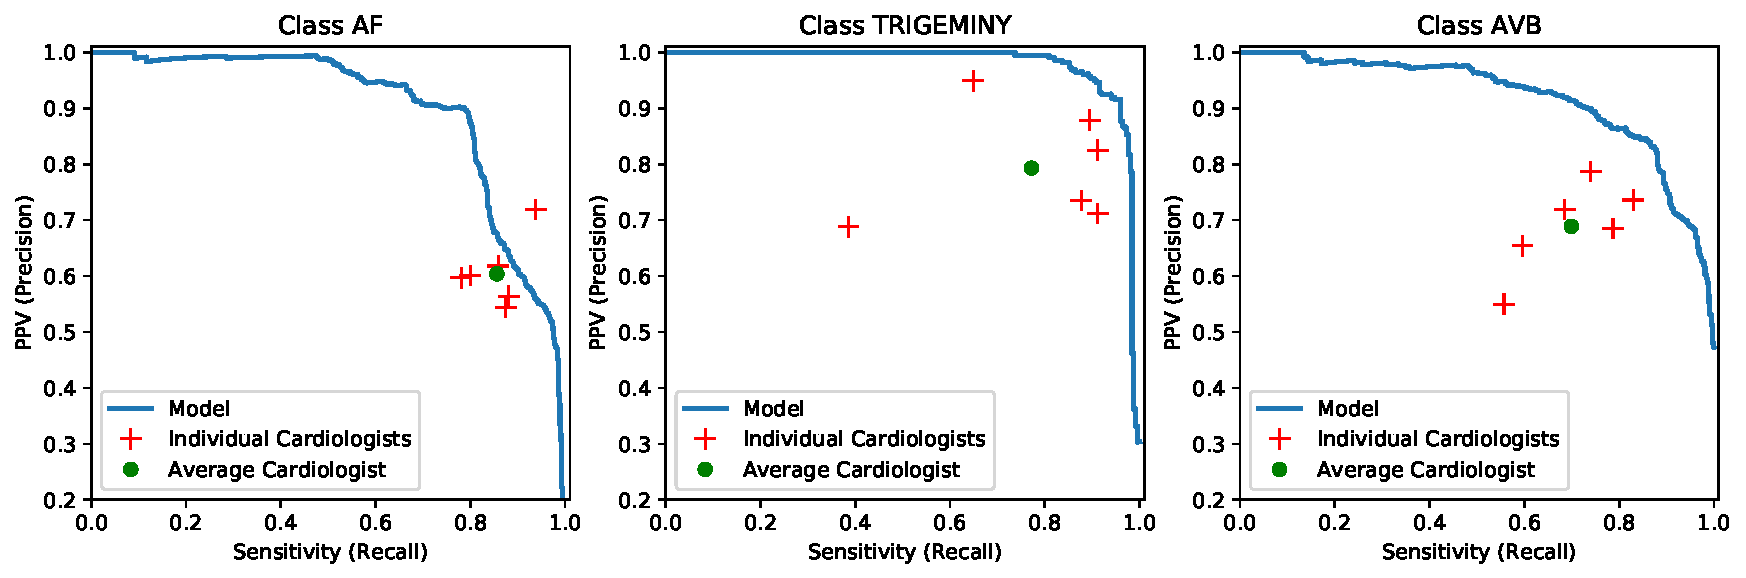
\includegraphics[width=1.0\textwidth]{arrhythmias/figures/prec_recall_curve.pdf}
    \caption{Precision-recall curves at the sequence level for atrial
    fibrillation and flutter (AF), trigeminy and atrioventricular block (AVB).}
\label{fig:arrhythmias:prec_recall_curve}
\end{figure}
